\begin{multicols}{2}
\section{Teorema Integral de Fresnel-Kirchoff}\label{sec: teo}

La difracción y los patrones de interferencia que produce pueden ser explicados a partir del \emph{principio de Huygens-Fresnel}:
\begin{quote}
	Cada punto en un frente de onda de luz puede ser tomado como una fuente secundaria de ondas esféricas, y el campo resultante más allá del frente es la superposición de estas ondas \parencite{pedrotti}.
\end{quote}

Sin embargo, el principio por sí solo no ofrece una explicación a porque no hay propagación opuesta a partir de las fuentes secundarias.

Este principio, y la ausencia de propagación opuesta, pueden ser obtenidos a partir del \emph{Teorema Integral de Kirchoff}. De este teorema no obtendremos una descripción completa del campo eléctrico difractado en un punto $\mathcal P$ después de atravesar una apertura, sino que nos limitaremos a estudiar la magnitud del campo eléctrico en $\mathcal P$. A esta aproximación se le conoce como la \textit{aproximación escalar}\parencite{fowles-1989}.

Partimos de una de las identidades de Green: sea $\Omega$ un subconjunto acotado de $\R^3$ y $\psi, \varphi \in C^2(\Omega)$.
\begin{multline}
	\int_{\partial \Omega} (\psi \nabla \varphi - \varphi \nabla \psi) \cdot d\vec S \\
	= \int_{\Omega} (\psi \nabla^2 \varphi - \varphi \nabla^2 \psi) \, dV.
\end{multline}

Como nos interesa estudiar ondas esféricas, resulta apropiado tomar a $\psi$ y $\varphi$ como ecuaciones de onda, es decir, que satisfacen
\begin{equation}
	\left (\nabla^2  - \frac{1}{c^2} \partial_t^2\right ) f = 0.
\end{equation}
Sustituyendo en la lado derecho de la identidad de Green
\begin{equation}\label{eq: time_Green}
	\frac{1}{c^2} \int_{\Omega} (\psi \, \partial_t^2 \varphi - \varphi  \,\partial_t^2 \psi) \, dV.
\end{equation}
Como en este trabajo empleamos ondas monocromáticas, podemos asumir que ambas funciones son separables como
\begin{equation}
	\psi(r, t) = \Psi(r) \eto{i\omega t}, \qquad \varphi(r, t) = \Phi(r) \eto{i\omega t}.
\end{equation}
Sustituyendo en \eqref{eq: time_Green},
\begin{multline}
	\frac{1}{c^2} \int_{\Omega} (\psi(r)\Phi(r) \cdot -\omega^2 \eto{i\omega t}\\
	 - \Phi(r)\psi(r) \cdot -\omega^2 \eto{i\omega t}) \, dV = 0.
\end{multline}

Es decir, si $\psi$ y $\varphi$ son funciones de onda monocromáticas, entonces
\begin{equation}\label{eq: Green}
	\int_{\partial \Omega} (\psi \nabla \varphi - \varphi \nabla \psi) \cdot d\vec S = 0.
\end{equation}
Para considerar a las ondas esféricas en $\mathcal P$, simplificamos los cálculos tomando a $\mathcal P$ como el origen de coordenadas y tomamos
\begin{equation}
	\varphi(r, t) = \varphi_0 \frac{\eto{i(kr + \omega t)}}{r}.
\end{equation}

Aunque $\varphi$ representa ahora ondas esféricas convergentes en $\mathcal P$, hay que aclarar que no tienen una realidad física en el fenómeno de difracción y solo resultan un artificio matemático útil para llegar a una expresión para $\psi$, que tomaremos como la \emph{perturbación óptica} en $\mathcal P$.

Antes de sustituir en \eqref{eq: Green}, debemos tomar una consideración extra a raíz de la forma de $\varphi$: como esta diverge en $\mathcal P$, debemos tomar a $\Omega$ como un sobconjunto acotado de $\R^3$ \emph{que no incluye al origen}, como se muestra en la figura~\ref{fig: integration}.

\begin{figure}[H]
	\centering
	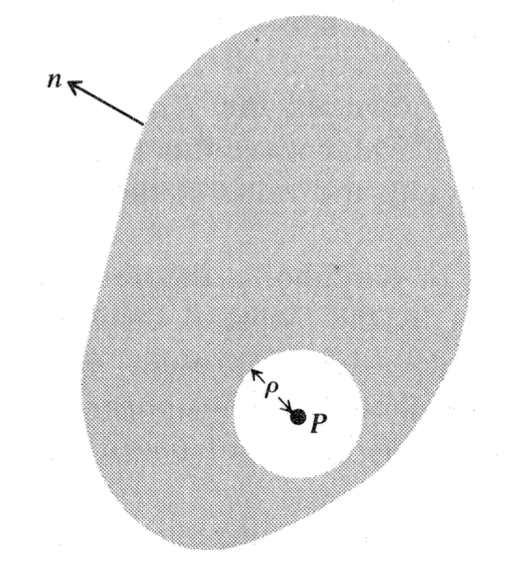
\includegraphics[width=.6\linewidth]{Imagenes/kirchoff}
	\caption{Se integra en una región que no contiene al punto $\mathcal P$. Imagen tomada de \parencite{fowles-1989}.}
	\label{fig: integration}
\end{figure}

 Procedemos entonces con una deducción similar a la de la ley de Gauss, es decir, en el interior de $\Omega$ colocamos una cavidad esférica de radio $\epsilon > 0$ centrada en el origen, a su superficie la denotamos por $\partial \Omega'$ mientras que a la superficie externa la seguimos tomando como $\partial \Omega$.

Como estas dos superficies son disjuntas, podemos escribir
\begin{multline}\label{eq: inner}
	\int_{\partial \Omega} (\psi \nabla \varphi - \varphi \nabla \psi) \cdot d\vec S \\
	+  \int_{\partial \Omega'} (\psi \nabla \varphi - \varphi \nabla \psi) \cdot d\vec S= 0.
\end{multline}
En $\partial \Omega'$, $\nabla = \univ{r} \partial r$ para $\psi, \varphi$. Calculamos $\nabla \varphi$.
\begin{equation}\label{eq: gradi}
	\nabla \varphi =  \varphi_0 \eto{i\omega t}\frac{\partial}{\partial r}\frac{\eto{ikr}}{r} \univ r
	= \left(ik - \frac{1}{r} \right)\varphi \univ r.
\end{equation}
La segunda integral de \eqref{eq: inner} se vuelve entonces
\begin{equation}
	 -\int_{\partial \Omega'} \left[\left(ik - \frac{1}{r} \right)\psi - \frac{\partial}{\partial r}\psi \right] \biggr\rvert_{r = \epsilon} \varphi \, \epsilon^2 d\Omega
\end{equation}
donde ha aparecido el signo negativo porque la normal a $\partial \Omega'$ es antiparalela a $\univ r$, y $d\Omega = d\theta^2 + \sen^2\theta d\phi^2$.

Si permitimos que $\epsilon \to 0$, entonces en el límite el único término que no se anula es
\begin{equation}
	\varphi_0 \eto{i(k\epsilon + \omega t)} \int_{\partial \Omega'} \psi \rvert_{r = \epsilon} \, d\Omega,
\end{equation}
y la integral converge a $4\pi \psi_{\mathcal P}$, es decir, el valor de $\psi$ en $\mathcal P$.

Sustituyendo en \eqref{eq: inner},
\begin{equation}
	\int_{\partial \Omega} (\psi \nabla \varphi - \varphi \nabla \psi) \cdot d\vec S + 4\pi \varphi_0 \eto{i\omega t}\psi_{\mathcal P} = 0,
\end{equation}
de lo que se obtiene inmediatamente, eliminando el factor común $\varphi_0 \eto{i\omega t}$, que
\begin{equation}\label{eq: kirchoff}
	\psi_{\mathcal P} = -\frac{1}{4\pi} \int_{\partial \Omega} \left (\psi \nabla \frac{\eto{ikr}}{r} - \frac{\eto{ikr}}{r}  \nabla \psi \right ) \cdot d\vec S.
\end{equation}

Esta expresión permite, así como la fórmula integral de Cauchy en variable compleja, calcular el valor de $\psi$ en un punto interior a una región $\Omega$ a a partir de sus valores y los de su derivada en la frontera.

\parencite{fowles-1989} aclara que $\psi$ no representa al campo eléctrico, como lo habíamos mencionado, por ser una cantidad escalar, y que $\abs{\psi}^2$ es una medida de la irradiancia $I$. Pero como en ondas monocromáticas $I \propto \norm{\vec E}^2$, podemos identificar entonces a $\psi$ con la magnitud del campo eléctrico en un punto dado.

Para aplicar \eqref{eq: kirchoff} para estudiar la difracción en aperturas arbitrarias, tomamos a $\partial \Omega$ como una superficie ubicada totalmente en el lado opuesto  de la barrera a la fuente $S$ y que incluye a la apertura (ver figura~\ref{fig: application}).

\begin{figure}[H]
	\centering
	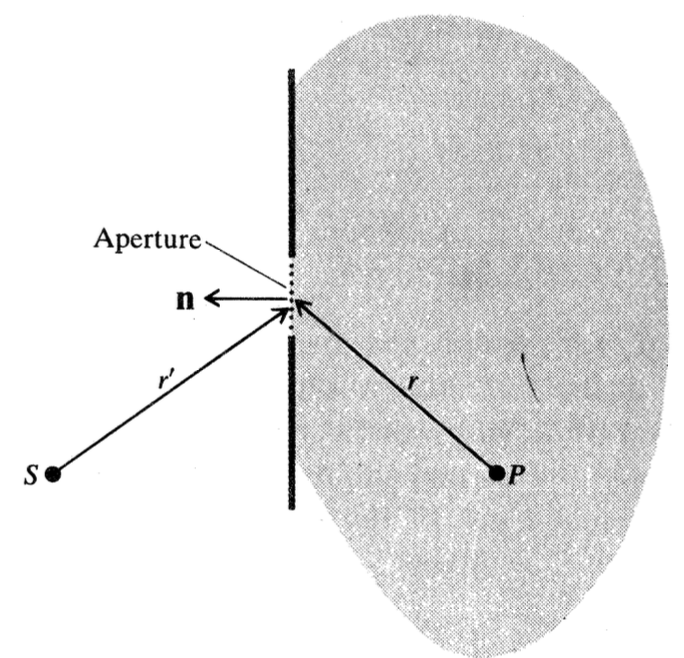
\includegraphics[width=.7\linewidth]{Imagenes/fresnel}
	\caption{Ondas emitidas desde $S$ atraviesan una apertura en una barrera y son transmitidas hasta el punto $\mathcal P$. Imagen tomada de \parencite{fowles-1989}.}
	\label{fig: application}
\end{figure}

Además, como consideramos que la barrera es opaca y que no transmite luz, podemos tomar que las ondas y sus derivadas que llegan a la apertura se anulan en toda la superficie $\partial \Omega$ exceptuando en la apertura $\mathcal A$. En la apertura, la onda $\psi$ es
\begin{equation}
	\psi = \psi_0\frac{\eto{i(kr' - \omega t)}}{r'}.
\end{equation}
Entonces
\begin{multline}
	\psi_{\mathcal P} = \frac{\psi_0 \eto{-i\omega t}}{4\pi} \int_{\mathcal A} \left (\frac{\eto{ikr}}{r}  \nabla \frac{\eto{ikr'}}{r'} \right.\\
	 \left. -  \frac{\eto{ikr'}}{r'}  \nabla \frac{\eto{ikr}}{r} \right ) \cdot d\vec S.
\end{multline}
Al calcular los gradientes en la integral obtenemos un resultado con la misma forma que en \eqref{eq: gradi}, solo sin la fase $i\omega t$. Cuando $r$ y $r'$ son mucho mayores que las longitudes de onda el término $\psi/r$ es despreciable y
\begin{equation}
	\psi_{\mathcal P} = \frac{ik \psi_0 \eto{-i\omega t}}{4\pi} \int_{\mathcal A} \frac{\eto{ik(r+r')}}{rr'}  (\univ r' - \univ r)
	  \cdot d\vec S.
\end{equation}
O en términos de la onda en $\mathcal A$
\begin{equation}\label{eq: almost}
	\psi_{\mathcal P} = -\frac{ik}{4\pi} \int_{\mathcal A} \frac{\eto{ikr}}{r}  (\univ r \cdot \univ n - \univ r' \cdot \univ n) \psi(r', t)\, dS.
\end{equation}
Esta integral puede entonces interpretarse como la suma ponderada de las contribuciones de ondas secundarias generadas en $\mathcal A$, es decir, es el enunciado matemático del principio de Huygens-Fresnel.

En nuestros experimentos, al estar la fuente alineada con el centro de la apertura $\univ r'$ y $\univ n$ apuntan siempre a lados opuestos de $\mathcal A$ y $\univ r' \cdot \univ n < 0$, mientras que $\univ r$ apunta al misma lado que $\univ n$. Es decir, $\univ r \cdot \univ n - \univ r' \cdot \univ n$ puede alcanzar su valor máximo.

Podemos considerar al punto $\mathcal P$ del mismo lado que $S$ sin alterar el análisis y como en este caso $\univ r$ y $\univ r'$ pueden apuntar en la misma dirección opuesta respecto a $\univ n$, el término $\univ r \cdot \univ n - \univ r' \cdot \univ n$ puede anularse, por lo que $\psi_{\mathcal P} = 0$ y no se mediría una perturbación óptica. Esto explica porque no hay una onda regresiva hacia la fuente.

Una observación adicional es que el término $-i$ produce un desfase de $\pi/2$ entre la onda incidente y la onda refractada.

\subsection{Difracción de Fraunhofer}
Por las simplificaciones matemáticas que implica considerar a las ondas incidentes sobre la apertura y a las que provienen de ella como planas, \parencite{hecht-1999} hace dos distinciones: cuando tanto la fuente como el punto de observación $\mathcal P$ están lo suficientemente alejados como para tomarlas como plana, se habla de \textit{difracción de Fraunhofer}, pero cuando ambos están tan cerca que se debe tomar en cuenta la curvatura de las ondas esféricas, se habla de \textit{difracción de Fresnel}. Nosotros estudiaremos la difracción de Fraunhofer.

En esta aproximación, \parencite{fowles-1989} toma las siguientes consideraciones: la distribución angular de la luz difractada es lo suficientemente pequeña para tomar a $\univ r \cdot \univ n - \univ r' \cdot \univ n$ como constante. Al estar la fuente lo suficientemente alejada podemos tomar $\psi(r', t)$ como constante respecto a $r'$, y finalmente, la variación en $\eto{ikr}/r$ se debe principalmente al factor exponencial, así que sustituimos en $1/r$ el valor medio $r_0$ de $r$.

Así, reuniendo en una constante $C$ las constantes obtenidas, la ecuación \eqref{eq: almost} se simplifica como
\begin{equation}
	\psi_{\mathcal P} = C \int_{\mathcal A} \eto{ikr} dS.
\end{equation}

Esta es la misma expresión que usa \parencite{hecht-1999}, aunque por un procedimiento menos formal.

\subsection{Difracción de una Rendija}\label{sec: una}

Tomamos primero el caso sencillo de una rendija de longitud $L$ a lo largo del eje $y$ y grosor $b$ a lo largo del eje $x$. Si $x$ es la distancia entre el centro de la rendija $r_0$ y un punto en ella, entonces $r = r_0 + x \sen \theta$, donde $\theta$ es el ángulo entre el centro del plano de observación y el punto de medición $\mathcal P$. Entonces
\begin{equation}\label{eq: one}
	\begin{split}
		\psi_{\mathcal P} &= C\eto{ikr_0} \int_{-b/2}^{b/2} \int_{-L/2}^{L/2} \eto{ik x \sen \theta} dy \, dx\\
		&= C L\eto{ikr_0}  \int_{-b/2}^{b/2}  \eto{ik x \sen \theta}  \, dx\\
		&= \frac{C L\eto{ikr_0}}{ik \sen \theta} \left(\eto{i\beta} - \eto{-i\beta} \right )\\
		&=  CLb\eto{ikr_0} \frac{\sen\beta}{\beta}.
	\end{split}
\end{equation}
Donde hemos tomado $\beta = kb \sen \theta /2$.
Definiendo $I_0 = \abs{CLb}^2$, calculamos la irradiancia en $\mathcal P$ como
\begin{equation}
	I(\theta) = \abs{\psi_\mathcal{P}}^2 = I_0 \left[ \frac{\sen \beta}{\beta}\right]^2.
\end{equation}

Esta ecuación describe entonces bandas oscuras en
\begin{equation}\label{eq: distance}
	\sen \theta = \frac{2}{kb} n\pi = \frac{n}{b}\lambda, \qquad n \in \mathbb Z \backslash\{0\},
\end{equation}
y como $\sen \alpha/\alpha \to 1$ cuando $\alpha \to 0$, en $\theta = 0$ existe la banda más brillante en lugar de una oscura.

A su vez, las bandas brillantes están localizadas en los extremos de la función $\sen \alpha/\alpha$, es decir, cuando se satisface
\begin{equation}
	\frac{d}{d\alpha} \frac{\sen \alpha}{\alpha} = \frac{\alpha \cos \alpha - \sen \alpha}{\alpha^2} = 0.
\end{equation}
La condición para los máximos es entonces
\begin{equation}
	\sen \theta = \frac{2}{kb} \tan \left( \frac{1}{2}kb \sen \theta \right ).
\end{equation}
Entonces, la irradiancia disminuye entre máximos como
\begin{equation}
\begin{split}
	&\frac{I(\theta_{n+1})}{I(\theta_n)}\\
	&= \frac{\sen^2(\beta_{n+1})/(\beta_{n+1})^2}{\sen^2\beta_n/\beta_n^2}\\
	&= \frac{\sen^2\beta_n}{\sen^2 \beta_{n+1}} \frac{\beta_{n+1}^2\cos^2(\beta_{n+1})}{\beta_n^2\cos^2\beta_n}\\
	&=   \frac{\cos^2\beta_{n+1}}{\cos^2\beta_n}.
\end{split}
\end{equation}
Por ejemplo, el primer máximo secundario ocurre cuando $\alpha = 1.43 \pi$.
\begin{equation}
	\frac{I(\theta_1)}{I_0} = \cos^2(1.43 \pi) = \num{.0476} = \qty{4.76}{\percent}.
\end{equation}
Y está localizado en
\begin{equation}
	\sen \theta = \frac{1.43}{b}\lambda.
\end{equation}
\begin{figure}[H]
	\centering
	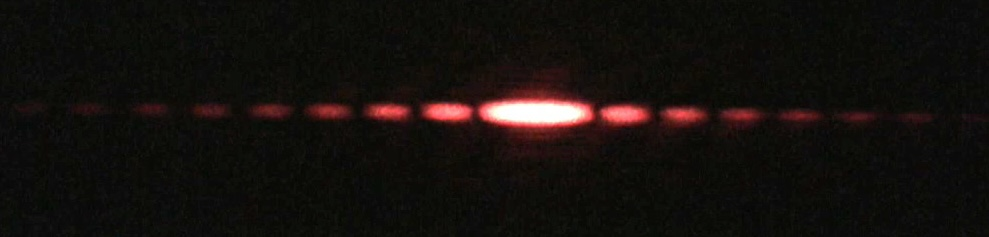
\includegraphics[width=.9\linewidth]{Imagenes/single-slit}
	\caption{Patrón de difracción de una sola rendija. Notése que, a diferencia de la figura \ref{fig: double_slit}, las bandas brillantes no están subdivididas. Imagen recuperada de \parencite{single_slit}.}
	\label{fig: single-slit}
\end{figure}

\subsection{Difracción Circular}
En esta situación tomamos una apertura ciruclar de radio $R$. La integral a resolver es
\begin{equation}
	\psi_\mathcal{P} = 2C\eto{ikr_0} \int_{-R}^R \eto{ik x \sen \theta} \sqrt{R^2 - x^2} \, dx.
\end{equation}
Simplificamos la expresión usando el cambio de variable $x = Ru$ y con la cantidad $\rho = kR \sen \theta$ a
\begin{equation}
	R^2\int_{-1}^1 \eto{i\rho u}\sqrt{1 - u^2} \, du = \frac{\pi J_1(\rho)}{\rho},
\end{equation}
donde $J_1$ es la función de Bessel de la primera especia, que satisface $\rho \to 0$ $J_1 \to 1/2$. Si definimos ahora $I_0 = (\pi CR^2)^2$,
\begin{equation}\label{eq: circular}
	I(\theta) = I_0 \left[\frac{2J_1(kR \sen \theta)}{kR \sen \theta} \right]^2.
\end{equation}

El primer cero de $J_1$ ocurre en $kR \sen \theta = 3.8317$. Esto nos da una expresión para la región circular más brillante, conocido como \emph{círculo de Airy}. Su apertura angular $\theta$ es
\begin{equation}\label{eq: airy}
	\sen \theta = \frac{3.8317}{kR} = \frac{3.8317}{2\pi R}\lambda = \frac{1.22}{D}\lambda,
\end{equation}
donde $D = 2R$ es el diámetro de la apertura circular.

\subsection{Difracción por Múltiples Rendijas}
Consideramos ahora una situación similar a la difracción en una rendija de la subsección \ref{sec: una}, donde tomamos ahora $N$ rendijas con una separación $a$ entre sus centros. 
La integral de la segunda igualdad de \eqref{eq: one} se sustituye por
\end{multicols}
\begin{equation}\label{eq: massive}
	\sum_{r=1}^{N/2} \left( \int_{-[(2r-1)a + b]/2}^{-[(2r-1)a - b]/2} \eto{ik x \sen \theta} dx + \int_{[(2r-1)a - b]/2}^{[(2r-1)a + b]/2} \eto{ik x \sen \theta} dx
	\right).
\end{equation}
\begin{figure}[H]
	\centering
	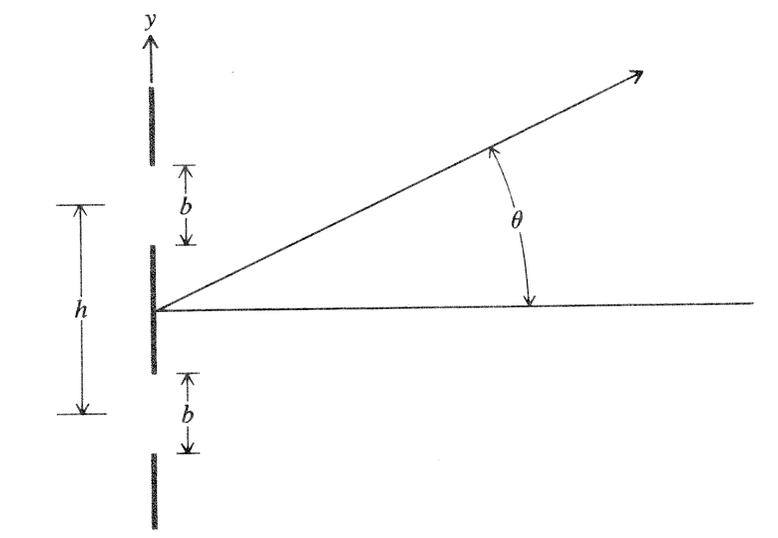
\includegraphics[width=.4\linewidth]{Imagenes/DS}
	\caption{El ángulo $\theta$ ahora se mide como la separación angular entre el punto $\mathcal P$ y el centro del arreglo de $N$ rendijas. Imagen tomada de \parencite{fowles-1989}.}
	\label{fig: DS}
\end{figure}

Manipulamos la primera integral para obtener
\begin{equation}
	\int_{-[(2r-1)a + b]/2}^{-[(2r-1)a - b]/2} \eto{ik x \sen \theta} dx 
	= -\int_{[(2r-1)a + b]/2}^{[(2r-1)a - b]/2} \eto{-ik x \sen \theta} dx
	= \int_{[(2r-1)a - b]/2}^{[(2r-1)a + b]/2} \eto{-ik x \sen \theta} dx.
\end{equation}
Sustituyendo en \eqref{eq: massive}
\begin{equation}
	\begin{split}
	&\sum_{r=1}^{N/2}   \int_{[(2r-1)a - b]/2}^{[(2r-1)a + b]/2} \left(
	\eto{ik x \sen \theta}  +  \eto{-ik x \sen \theta}
	\right) dx
	= 2\sum_{r=1}^{N/2}   \int_{[(2r-1)a - b]/2}^{[(2r-1)a + b]/2} 
	\cos(k x \sen \theta)dx\\
	&=\frac{2}{k\sen \theta}\sum_{r=1}^{N/2}\left [ \sen\left( \frac{(2r-1)a + b}{2}k\sen \theta \right) - \sen\left( \frac{(2r-1)a - b}{2}k\sen \theta \right)
	\right].
	\end{split}
\end{equation}
Definimos $\alpha = ka \sen \theta /2$.
\begin{equation}
	\begin{split}
		&\frac{b}{\beta}\sum_{r=1}^{N/2}\left [ \sen\left( \frac{(2r-1)a + b}{2}k\sen \theta \right) - \sen\left( \frac{(2r-1)a - b}{2}k\sen \theta \right)
	\right]\\
	&= \frac{b}{\beta}\sum_{r=1}^{N/2}\left [ \sen \bigl( (2r-1)\alpha + \beta \bigr) -  \sen \bigl( (2r-1)\alpha - \beta \bigr)
	\right]\\
	&= \frac{b}{\beta} \sum_{r=1}^{N/2} 2 \cos\bigl((2r-1)\alpha \bigr) \sen \beta
	= \frac{2b\sen \beta}{\beta} \sum_{r=1}^{N/2} \cos [(2r-1)\alpha ]\\
	&= \frac{2b\sen \beta}{\beta} \Re\left( \sum_{r=1}^{N/2 - 1} \eto{i(2r+1)\alpha } \right)
	=  \frac{2b\sen \beta}{\beta} \Re \left[  \eto{i\alpha} \sum_{r=0}^{N/2 - 1} \left(\eto{2i \alpha} \right)^r \right]\\
	&= \frac{2b\sen \beta}{\beta} \Re \left[ \eto{i\alpha}\frac{1 - \eto{iN\alpha}}{1 - \eto{2i\alpha}} \right]
	= \frac{2b\sen \beta}{\beta} \Re \left[\frac{\eto{iN\alpha} - 1}{\eto{i\alpha} - \eto{-i\alpha}} \right]\\
	&= \frac{2b\sen \beta}{\beta} \Re \left[\frac{\cos(N\alpha) - 1 + i \sen(N\alpha)}{2i \sen \alpha} \right]\\
	&=  b\frac{\sen \beta}{\beta} \frac{\sen (N\alpha)}{\sen \alpha}.
	\end{split}
\end{equation}
\begin{multicols}{2}
Entonces
\begin{equation}
	\psi_\mathcal{P} = CL\eto{ikr_0}  b\frac{\sen \beta}{\beta} \frac{\sen (N\alpha)}{\sen \alpha}.
\end{equation}
Definiendo $I_0 = \abs{CLb}^2$,
\begin{equation}\label{eq: multiple}
	I_N(\theta) = I_0 \left( \frac{\sen \beta}{\beta}\right)^2 \left[ \frac{\sen (N\alpha)}{\sen \alpha}\right]^2.
\end{equation}
Si tomamos $N=1$ recuperamos la ecuación \eqref{eq: one}, por lo que podemos identificar a $(\sen \beta/\beta)^2$ como el factor de difracción causado por cada rendija, mientras que $[\sen(N\alpha)/\sen \alpha]^2$ debe entonces representar la interferencia de las $N$ rendijas.

De \eqref{eq: multiple} podemos obtener inmediatamente la irradiancia para una doble rendija
\begin{equation}
\begin{split}
	I_2(\theta) &= I_0 \left( \frac{\sen \beta}{\beta}\right)^2 \left[ \frac{\sen (2\alpha)}{\sen \alpha}\right]^2\\
	&= 4I_0  \left( \frac{\sen \beta}{\beta}\right)^2 \cos^2\alpha.
\end{split}
\end{equation}
Notamos que la irradiancia máxima para la doble rendija es cuatro veces la de una individual. A su vez, el factor de interferencia $\cos^2 \alpha$ explica porque en la imagen \ref{fig: double_slit} las bandas brillantes están subdivididas mientras que en la figura \ref{fig: single-slit} no lo están.

En el laboratorio nosotros medimos la distancia entre los centros de las bandas brillantes, por lo que la expresión útil para nuestros objetivos es
	\begin{equation}\label{eq: maxima}
		\sen \theta = \frac{2n\pi}{ka} = \frac{n}{a}\lambda.
	\end{equation}
\end{multicols}
\begin{figure}[htb!]
	\centering
	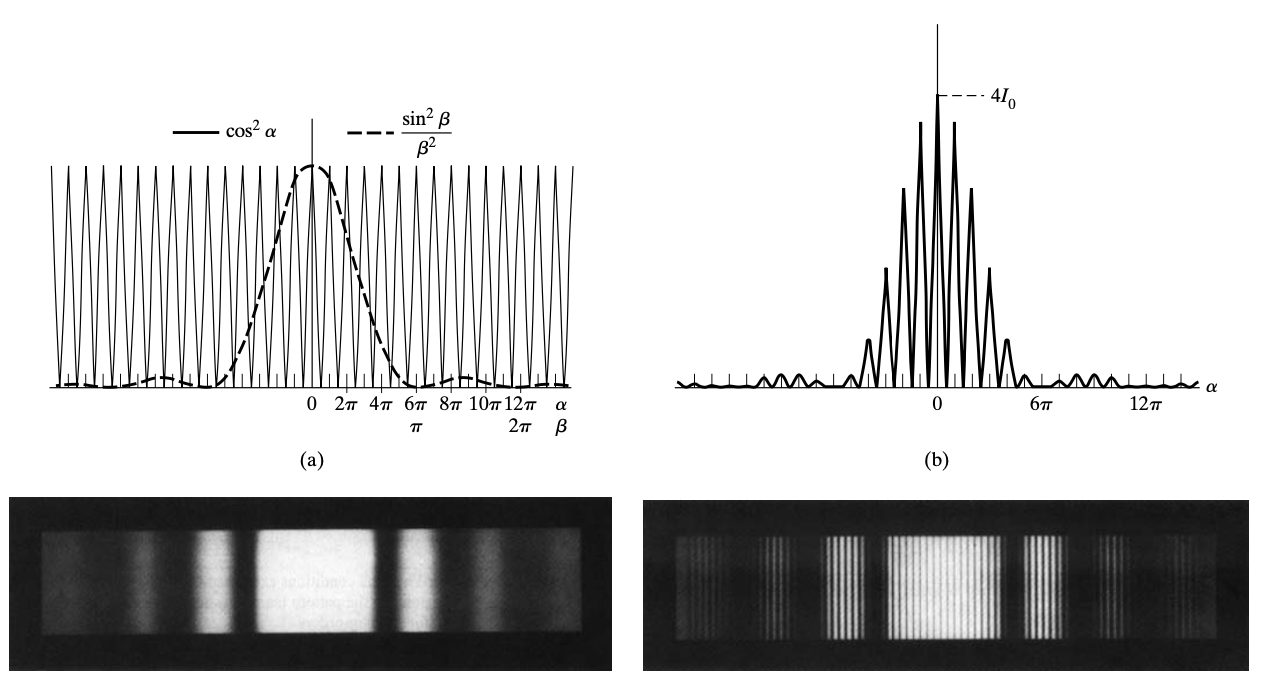
\includegraphics[width=.7\linewidth]{Imagenes/compare}
	\caption{Las dos imágenes superiores ilustran la irradiancia producida por una doble rendija, y las dos imágenes inferiores comparan los patrones de difracción de una sola rendija y de dos rendijas. Imagen recuperada de \parencite{pedrotti}.}
	\label{fig: compare}
\end{figure}
